% =====================================================================
%  MẪU BÁO CÁO BÀI TẬP 1 — Giới thiệu ngành Trí tuệ Nhân tạo (CSC00006)
%  "Chân dung trợ lý AI"
% ---------------------------------------------------------------------
%  CÁCH DÙNG
%  1. Overleaf: New Project -> Upload Project -> chọn file zip này.
%     Menu -> Compiler: pdfLaTeX. Bấm Recompile.
%  2. Chọn hướng làm ở dòng \huongBtrue bên dưới (mặc định: Hướng A).
%  3. Thay mọi chỗ <...> bằng nội dung CỦA BẠN. Ảnh để trong images/.
%  4. Các nhãn [YC1]..[YC10] đánh dấu chỗ đáp ứng 10 yêu cầu kỹ thuật
%     ở mục 3 đề bài. Trước khi nộp, dò lại đủ 10 nhãn là yên tâm.
%  5. Khi xong, có thể xoá nhánh của hướng bạn KHÔNG làm cho gọn.
% =====================================================================
\documentclass[12pt,a4paper]{article}

% ---------- Tiếng Việt (pdfLaTeX) ----------
\usepackage[utf8]{inputenc}
\usepackage[T5]{fontenc}
\usepackage[vietnamese]{babel}

% ---------- Trình bày ----------
\usepackage[margin=2.5cm]{geometry}
\usepackage{amsmath,amssymb}
\usepackage{graphicx}          % \includegraphics
\usepackage{booktabs}          % \toprule \midrule \bottomrule
\usepackage{float}             % [H] = đặt hình/bảng đúng chỗ
\usepackage{pgfplots}          % vẽ biểu đồ (Hướng B)
\pgfplotsset{compat=1.18}
\usepackage[hidelinks]{hyperref} % \url, link bấm được trong PDF
\graphicspath{{images/}}

% ---------- CHỌN HƯỚNG ----------
\newif\ifhuongB
% \huongBtrue   % <-- Làm Hướng B? Xoá dấu % ở ĐẦU dòng này.

\begin{document}

% =====================================================================
% [YC1] TRANG BÌA
% =====================================================================
\begin{titlepage}
  \centering
  {\large TRƯỜNG ĐẠI HỌC KHOA HỌC TỰ NHIÊN -- ĐHQG-HCM\\
   KHOA CÔNG NGHỆ THÔNG TIN\par}
  \vspace{3.5cm}
  {\Large\bfseries BÁO CÁO BÀI TẬP 1\par}
  \vspace{0.3cm}
  {\large Môn: Giới thiệu ngành Trí tuệ Nhân tạo (CSC00006)\par}
  \vspace{1.2cm}
  \ifhuongB
    {\huge\bfseries Đọ sức chatbot:\\ <Chatbot 1> vs <Chatbot 2>\par}
  \else
    {\huge\bfseries Chân dung trợ lý AI:\\ <Tên công cụ>\par}
  \fi
  \vfill
  \begin{tabular}{rl}
    Sinh viên: & <Họ và tên> \\
    MSSV:      & <MSSV> \\
    Lớp:       & <Lớp> \\
    Giảng viên:& Trần Huy Bân \\
  \end{tabular}
  \par\vspace{1.5cm}
  TP. Hồ Chí Minh, \today
\end{titlepage}

% =====================================================================
% [YC2] TÓM TẮT + MỤC LỤC TỰ ĐỘNG
% =====================================================================
\begin{abstract}
<Viết 4--6 câu: bạn tìm hiểu công cụ nào / so sánh những chatbot nào,
làm bằng cách nào, và phát hiện quan trọng nhất là gì.
Viết phần này SAU CÙNG.>
\end{abstract}

\tableofcontents
\newpage

\ifhuongB
% #####################################################################
%                              HƯỚNG B
%                       Đọ sức chatbot
% #####################################################################

% [YC3] Ít nhất 3 mục lớn (\section), có mục con (\subsection)
\section{Giới thiệu}
<Vì sao bạn muốn so sánh các chatbot này? Bạn kỳ vọng gì trước khi làm?>%
\footnote{<Chú thích chân trang, ví dụ: phiên bản chatbot bạn dùng
và ngày thử nghiệm.>}  % [YC8] chú thích chân trang

\section{Phương pháp}
\subsection{Công cụ được so sánh}
% [YC4] danh sách không thứ tự
\begin{itemize}
  \item \textbf{<Chatbot 1>}: <phiên bản, gói miễn phí/trả phí>.
  \item \textbf{<Chatbot 2>}: <...>.
  \item \textbf{<Chatbot 3>} (nếu có): <...>.
\end{itemize}

\subsection{Bộ câu hỏi}
Bảng~\ref{tab:cauhoi} liệt kê 5 câu hỏi lấy từ các môn mình đang học.

% [YC5] bảng có chú thích
\begin{table}[H]
  \centering
  \caption{Bộ 5 câu hỏi thử nghiệm}
  \label{tab:cauhoi}
  \begin{tabular}{clp{8cm}}
    \toprule
    \# & Loại & Nội dung câu hỏi (tóm tắt) \\
    \midrule
    1 & Tính toán        & <Câu hỏi Giải tích / Đại số...> \\
    2 & Khái niệm        & <...> \\
    3 & Code ngắn        & <...> \\
    4 & Tiếng Việt / VH  & <...> \\
    5 & Câu bẫy          & <Câu hỏi có tiền đề sai...> \\
    \bottomrule
  \end{tabular}
\end{table}

\subsection{Quy trình và cách chấm}
% [YC4] danh sách có thứ tự
\begin{enumerate}
  \item Hỏi y hệt nhau trên từng chatbot, mỗi câu một hội thoại mới.
  \item Chấm mỗi câu theo thang 0--1--2
        (0: sai; 1: đúng một phần; 2: đúng và giải thích rõ).
  \item Tính điểm trung bình theo công thức~\eqref{eq:tb}.
\end{enumerate}

% [YC7] công thức: inline $...$ và công thức đánh số (equation)
Gọi $s_{k,i} \in \{0,1,2\}$ là điểm của chatbot $k$ ở câu $i$.
Điểm trung bình của chatbot $k$ là
\begin{equation}
  \bar{S}_k = \frac{1}{5}\sum_{i=1}^{5} s_{k,i}.
  \label{eq:tb}
\end{equation}

\section{Kết quả}
Bảng~\ref{tab:diem} là điểm chi tiết; Hình~\ref{fig:bieudo}
so sánh điểm trung bình.   % [YC8] tham chiếu chéo \ref

\begin{table}[H]
  \centering
  \caption{Điểm từng câu của các chatbot}
  \label{tab:diem}
  \begin{tabular}{lccc}
    \toprule
    Câu hỏi & <Chatbot 1> & <Chatbot 2> & <Chatbot 3> \\
    \midrule
    Câu 1 & 2 & 1 & 2 \\
    Câu 2 & 2 & 2 & 1 \\
    Câu 3 & 1 & 2 & 2 \\
    Câu 4 & 2 & 0 & 2 \\
    Câu 5 & 1 & 1 & 2 \\
    \midrule
    Trung bình $\bar{S}_k$ & 1.6 & 1.2 & 1.8 \\
    \bottomrule
  \end{tabular}
\end{table}

% [YC6] hình có chú thích — biểu đồ vẽ bằng pgfplots
% Thay các số (A,1.6) ... bằng điểm thật của bạn.
\begin{figure}[H]
  \centering
  \begin{tikzpicture}
    \begin{axis}[ybar, ymin=0, ymax=2.3, ytick={0,0.5,...,2}, bar width=24pt,
        width=0.6\textwidth, height=5.5cm,
        symbolic x coords={A,B,C}, xtick=data,
        ylabel={Điểm trung bình}, nodes near coords]
      \addplot coordinates {(A,1.6) (B,1.2) (C,1.8)};
    \end{axis}
  \end{tikzpicture}
  \caption{Điểm trung bình của các chatbot (A: <...>, B: <...>, C: <...>)}
  \label{fig:bieudo}
\end{figure}

% [YC6] ảnh chụp màn hình THẬT của bạn (bỏ vào images/)
Hình~\ref{fig:caubay} là câu trả lời của <Chatbot> cho câu bẫy.
\begin{figure}[H]
  \centering
  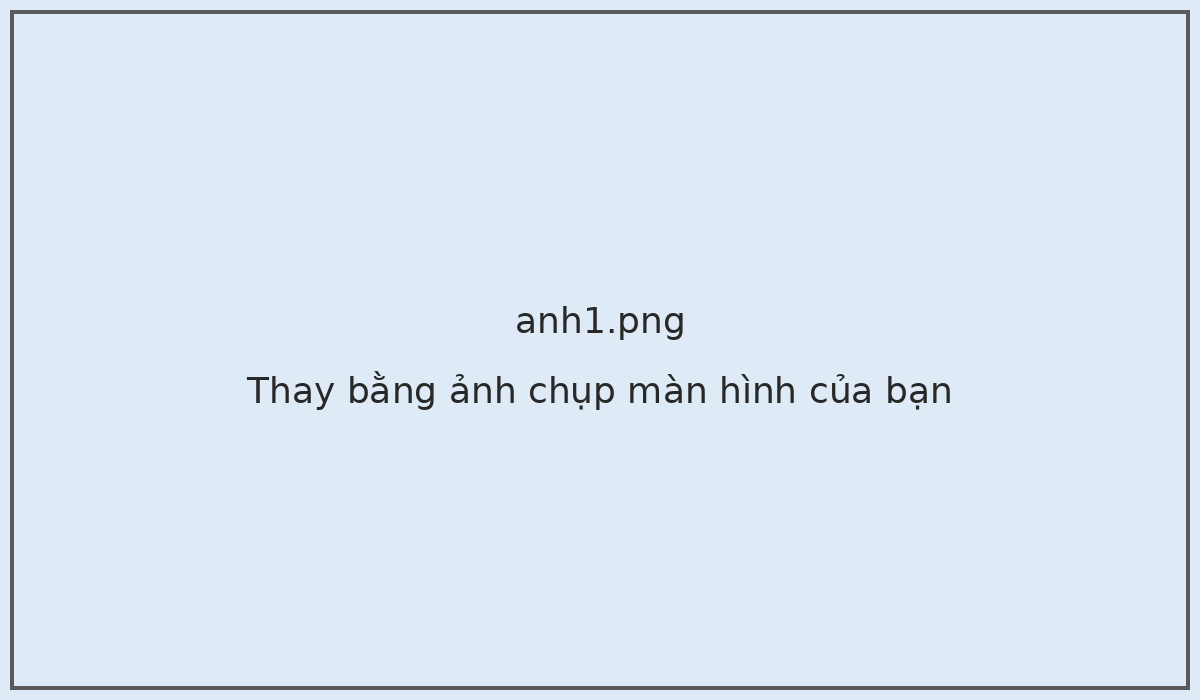
\includegraphics[width=0.75\textwidth]{anh1.png}
  \caption{<Chatbot> trả lời câu hỏi số 5 (câu bẫy)}
  \label{fig:caubay}
\end{figure}

\section{Thảo luận}
<Chatbot nào tốt hơn ở loại câu hỏi nào? Vì sao bạn nghĩ vậy?
Có câu nào tất cả đều sai không? Kết quả có khớp kỳ vọng ban đầu?>

Theo~\cite{vaswani2017}, <...>.   % [YC9] trích dẫn tài liệu

\section{Kết luận}
<2--4 câu: điều bạn rút ra, và bạn sẽ dùng chatbot thế nào khi học.>

\else
% #####################################################################
%                              HƯỚNG A
%                     Hồ sơ một công cụ AI
% #####################################################################

% [YC3] Ít nhất 3 mục lớn (\section), có mục con (\subsection)
\section{Giới thiệu}
<Vì sao bạn chọn công cụ này? Bạn dùng nó vào việc gì hằng ngày?>%
\footnote{<Chú thích chân trang, ví dụ: phiên bản bạn đang dùng.>}
% ^ [YC8] chú thích chân trang

\section{Nguồn gốc}
<Công ty phát triển, thời điểm ra mắt.> Bảng~\ref{tab:mocs} tóm tắt
các cột mốc chính.   % [YC8] tham chiếu chéo \ref

% [YC5] bảng có chú thích
\begin{table}[H]
  \centering
  \caption{Các cột mốc chính của <Tên công cụ>}
  \label{tab:mocs}
  \begin{tabular}{lp{10cm}}
    \toprule
    Thời điểm & Sự kiện \\
    \midrule
    <tháng/năm> & <Ra mắt phiên bản đầu tiên> \\
    <tháng/năm> & <...> \\
    <tháng/năm> & <...> \\
    \bottomrule
  \end{tabular}
\end{table}

\section{Cách hoạt động ở mức khái niệm}
\subsection{Mô hình ngôn ngữ lớn là gì?}
<Giải thích bằng lời của bạn: LLM là gì, ``token'' là gì.>

\subsection{Đoán từ tiếp theo}
% [YC7] công thức: inline $...$ và công thức đánh số (equation)
Mô hình tính xác suất của một câu $w_1, w_2, \dots, w_n$ bằng cách nhân
xác suất của từng token khi biết các token đứng trước, xem~\eqref{eq:lm}:
\begin{equation}
  P(w_1,\dots,w_n) = \prod_{t=1}^{n} P(w_t \mid w_1,\dots,w_{t-1}).
  \label{eq:lm}
\end{equation}
Xác suất cho từng token tiếp theo thường tính bằng hàm softmax:
\begin{equation}
  P(w_t = i \mid \cdot) = \frac{e^{z_i}}{\sum_{j=1}^{|V|} e^{z_j}},
  \label{eq:softmax}
\end{equation}
trong đó $z_i$ là ``điểm'' mô hình gán cho token $i$ và $|V|$ là kích
thước bộ từ vựng. Nền tảng của các mô hình này là kiến trúc
Transformer~\cite{vaswani2017}.   % [YC9] trích dẫn tài liệu

\section{Tính năng và các gói sử dụng}
<Mô tả ngắn các tính năng chính.>
% [YC4] danh sách không thứ tự
\begin{itemize}
  \item <Tính năng 1>
  \item <Tính năng 2>
\end{itemize}

\begin{table}[H]
  \centering
  \caption{So sánh gói miễn phí và trả phí (tra cứu ngày <dd/mm/yyyy>)}
  \label{tab:goi}
  \begin{tabular}{lll}
    \toprule
    Tiêu chí & Miễn phí & Trả phí \\
    \midrule
    Giá / tháng    & 0 & <...> \\
    Mô hình dùng   & <...> & <...> \\
    Giới hạn       & <...> & <...> \\
    \bottomrule
  \end{tabular}
\end{table}

\section{Trải nghiệm của mình}
% [YC6] ít nhất 2 hình — ảnh chụp màn hình THẬT của bạn trong images/
Hình~\ref{fig:tot} là một ví dụ công cụ làm tốt, còn Hình~\ref{fig:sai}
là một lần nó trả lời sai hoặc ``bịa''.

\begin{figure}[H]
  \centering
  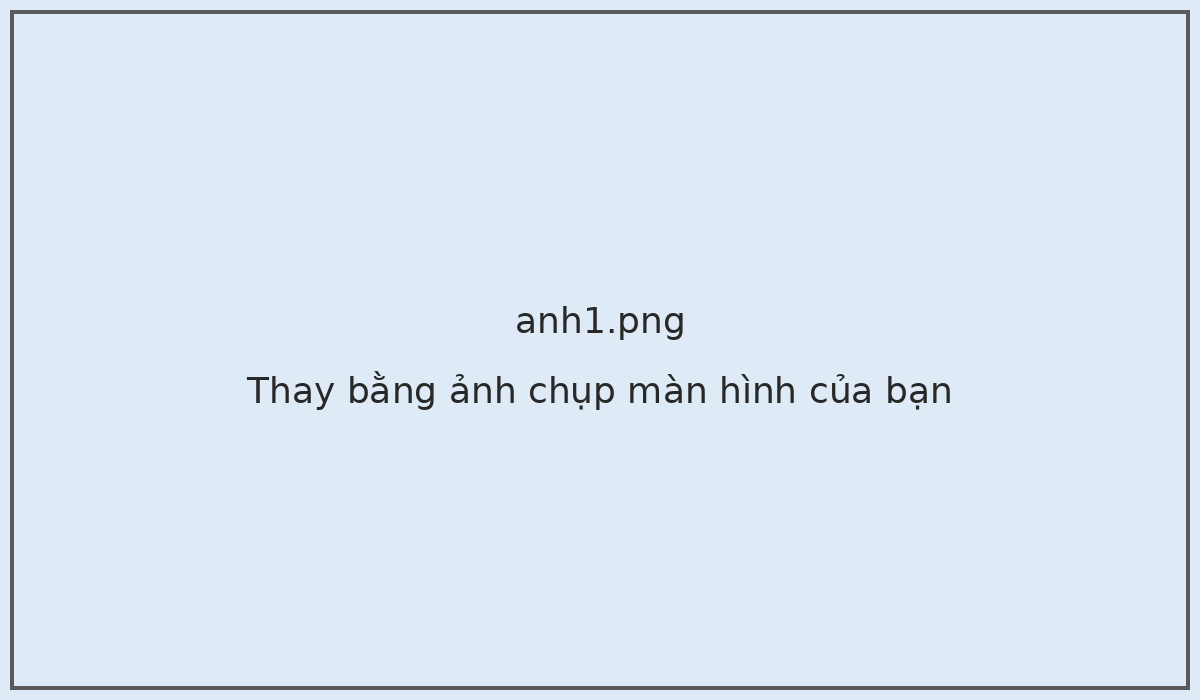
\includegraphics[width=0.75\textwidth]{anh1.png}
  \caption{<Mô tả: công cụ làm tốt việc gì>}
  \label{fig:tot}
\end{figure}

\begin{figure}[H]
  \centering
  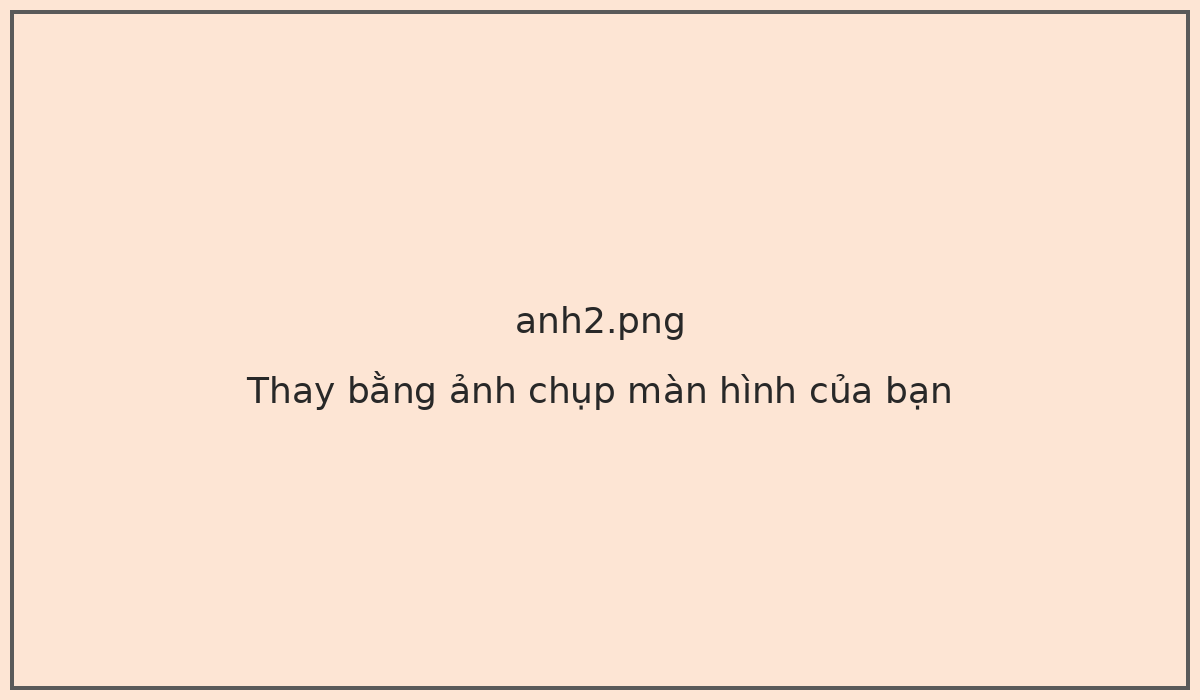
\includegraphics[width=0.75\textwidth]{anh2.png}
  \caption{<Mô tả: công cụ trả lời sai ở đâu>}
  \label{fig:sai}
\end{figure}

<Nhận xét của bạn về hai ví dụ trên.>

\section{Hạn chế và dùng có trách nhiệm}
% [YC4] danh sách có thứ tự
\begin{enumerate}
  \item \textbf{Hallucination:} <...>
  \item \textbf{Quyền riêng tư dữ liệu:} <...>
  \item \textbf{Quy định dùng AI trong học tập:} <...>
\end{enumerate}

\section{Kết luận}
<Bạn sẽ dùng công cụ này thế nào trong 4 năm đại học?>

\fi

% =====================================================================
% [YC9] TÀI LIỆU THAM KHẢO — ít nhất 4 nguồn CÓ THẬT, khai báo trong refs.bib
% Chỉ nguồn nào được \cite{...} mới hiện ra trong danh sách.
% Muốn liệt kê nguồn chưa cite trong bài: dùng \nocite{khoa}.
% =====================================================================
\nocite{brown2020,openai-chatgpt,ouyang2022}  % <-- thay bằng khoá của bạn
\bibliographystyle{plain}
\bibliography{refs}

% =====================================================================
% PHỤ LỤC BẮT BUỘC: NHẬT KÝ SỬ DỤNG AI
% =====================================================================
\appendix
\section{Nhật ký sử dụng AI}
% Không dùng AI? Xoá bảng, ghi: "Không sử dụng AI."
\begin{table}[H]
  \centering
  \begin{tabular}{p{4.2cm}p{5cm}p{5cm}}
    \toprule
    Prompt / link hội thoại & AI giúp phần nào & Mình đã sửa lại gì \\
    \midrule
    <``Sửa lỗi biên dịch này...''> & <Chỉ ra lỗi thiếu \texttt{\}}> & <...> \\
    <\url{https://...}>             & <...>                            & <...> \\
    \bottomrule
  \end{tabular}
\end{table}

\end{document}
% [YC10] Trước khi nộp: tạo project mới trên Overleaf, upload file zip
% MSSV.zip, bấm Recompile — chạy được, không lỗi mới nộp.
